\section{Capture de mouvement}
Dans cette partie, nous allons voir trois grandes classes de système de capture : système mécanique, système magnétique et système optique\cite{kn07}\cite{zo12}. Nous allons d'abord décrire les deux premiers systèmes. Ensuite, nous nous attarderons sur les systèmes optiques en regardant les systèmes optiques avec marqueurs et la \emph{Kinect} puis nous comparerons les performances des deux systèmes. L'étude se limite à ces deux dispositifs car sont ceux disponibles pendant mon stage.
\subsection{Système mécanique}
 Le système mécanique utilise un exosquelette (Voir Figure \ref{fig7}) qui doit être porté par la personne dont on capture le mouvement. Le mouvement est mesuré grâce à des potentiomètres qui sont placés au niveau des articulations ce qui simplifie le traitement de l'information. Son champ d'action est très grand car il n'est relié à aucun appareil externe et il n'y a pas de perturbation au niveau de la mesure. Par contre ce système est très intrusif car l'exosquelette encombre énormément la personne et l'empêche de faire des mouvements rapides.
 \begin{figure}[!h]
    	\centerline{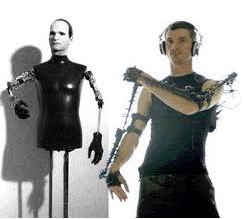
\includegraphics[scale=0.8]{./captureMecaTest}}
    	\caption{\label{fig7} Exemple d'exosquelette}
 \end{figure}
 %\newpage
\subsection{Système magnétique}
Pour ce système, des capteurs sensibles à un champ magnétique produit par un émetteur sont posés sur la personne (Voir Figure \ref{fig9}). La positon et l'orientation des capteurs sont mesurables et la vitesse d'acquisition est très rapide. Ce dispositif est assez peu encombrant par contre il est très sensible à des perturbations pouvant être créées par des objets métalliques ce qui crée des contraintes sur l'environnement où est utilisé ce système.
\begin{figure}[!h]
   	\centerline{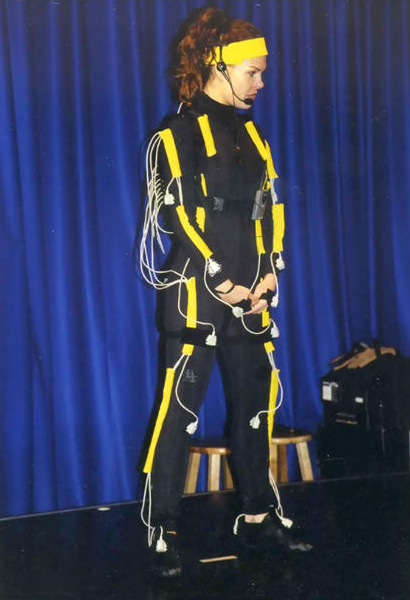
\includegraphics[scale=0.4]{./magne}}
   	\caption{\label{fig9} Combinaison d'un système magnétique}
\end{figure}
\subsection{Système optique}

\subsubsection{Système avec marqueurs}
Dans ce système, l'utilisateur porte une combinaison possédant des marqueurs réfléchissants (Voir Figure \ref{fig5}). Gr\^{a}ce à plusieurs caméras infrarouge, la position de chaque marqueur est récupérée en 3D. Pour cela, chaque caméra émet une lumière infrarouge qui va être réfléchie par le marqueur permettant ainsi d'obtenir une image 2D de celui-ci. En combinant les différentes images obtenues, la position 3D du marqueur peut être calculée. Ce système permet d'avoir une bonne précision et de capturer des mouvements rapides. Ce système est moins encombrant que les deux précédents.
\begin{figure}[!h]
   	\centerline{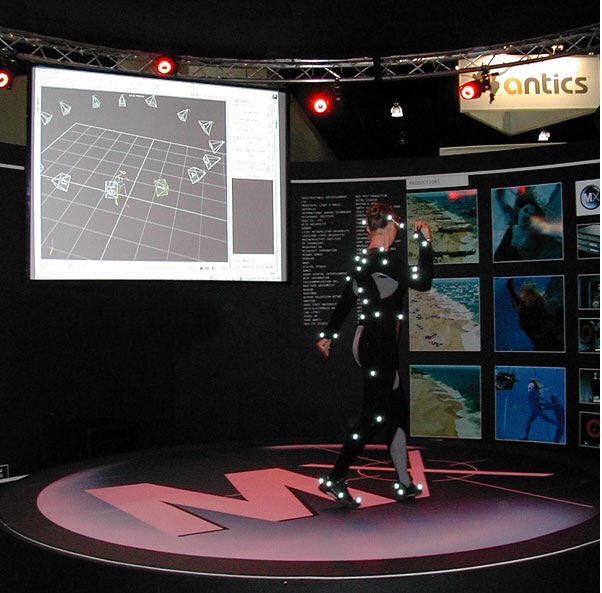
\includegraphics[scale=0.35]{./captureoptic}}
   	\caption{\label{fig5} Dispositif de système optique avec marqueurs}
\end{figure}
\subsubsection{\emph{Kinect}}
La \emph{Microsoft Kinect} est un système de capture de mouvement ne nécessitant pas de marqueurs et embarquant notamment une camera RGB et un capteur de profondeur \cite{ze12}. Le capteur de profondeur permet, en utilisant des rayons infrarouges, d'obtenir l'image de la scène en prenant en compte la profondeur (Voir Figure \ref{fig6}). L'image obtenue est traitée et les formes sont reconnues ce qui permet d'appliquer un squelette sur les formes humaines et ainsi suivre les mouvements.
\begin{figure}[!h]
   	\centerline{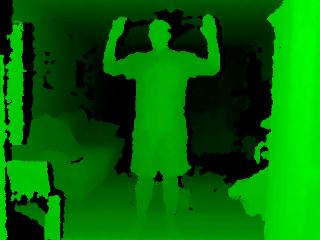
\includegraphics[scale=1.0]{./depthsensor}}
   	\caption{\label{fig6} Exemple d'image obtenu avec le capteur de profondeur}
\end{figure}
\subsubsection{Performances}
Dans l'article \cite{ch12}, les auteurs cherchent à comparer les performances obtenues avec un système optique avec marqueurs \emph{OptiTrack} et la \emph{Kinect} pour leur application d'aide à la réadaptation physique. Dans leur test, le sujet doit effectuer divers mouvements au niveau des mains, des coudes et des épaules qui sont capturés en même temps par le système \emph{OptiTrack} et le système \emph{Kinect}. Ils ont pu constater que la \emph{Kinect} capture très mal les mouvements effectués au niveau des épaules contrairement au système optique avec marqueurs. Cela est dû au fait que la \emph{Kinect} n'utilise qu'une seule caméra contrairement à l'autre système qui en utilise plusieurs (16 dans ce test). En comparant les trajectoires obtenues pour les coudes et mains, ils ont pu voir que les résultats des deux systèmes étaient proches. La latence relative entre les deux systèmes a également été calculée et le système \emph{OptiTrack} était plus rapide de 50 ms. La \emph{Kinect} n'offre pas la possibilité de reconnaitre la position et le mouvement des doigts. La portée de la \emph{Kinect} est d'environ de 0.5 à 4 mètres et la portée optimale est d'environ 1.2 à 3.5 mètres. La distance à laquelle se tient l'utilisateur influence beaucoup la performance du \emph{Kinect} \cite{li12}.

\subsection{Bilan}
Les systèmes optiques avec marqueurs sont rapides et permettent une bonne précision ce qui est nécessaire pour notre projet. Cependant ce système implique le port d'une combinaison avec marqueurs et cela pourrait gêner les utilisateurs dans notre contexte. Comme on a pu le voir, la \emph{Kinect}, bien qu'ayant des performances inférieures à ceux des systèmes optiques avec marqueurs, est suffisamment fiable et rapide. Par contre, la \emph{Kinect} peut ne pas capturer certains mouvements dû à sa seule caméra. Il faudra donc penser au placement de la caméra lors de la capture. Comme la \emph{Microsoft Kinect} est un dispositif plus simple à mettre en place, elle peut être utilisée dans plus d'environnements qu'un système optique avec marqueurs.